\problemname{Popp}

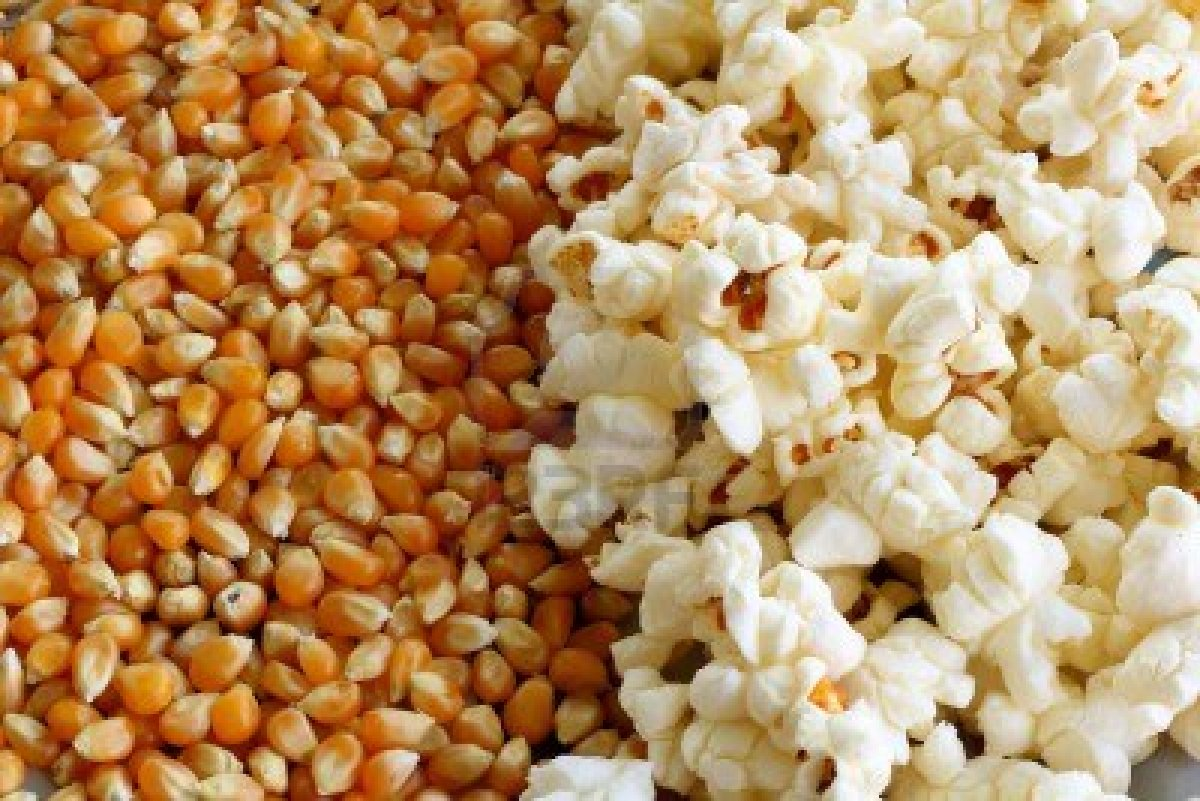
\includegraphics[width=0.4\textwidth]{popp.jpg}

Vignir litli á gott kvöld í vændum. Hann ætlar að poppa popp og horfa svo á
uppáhalds kvikmyndina sína, sem er auðvitað The Matrix. Hann fer fram í eldhús,
tekur fram pott, og kveikir á eldavélinni. Vigni er mjög annt um poppið sitt,
og leggur sig allan fram við að elda það rétt.

Hann byrjar á að taka saman $n$ popp-baunir, og skoðar svo hverja þeirra vel og
vandlega. Fyrir hverja popp-baun skrifar Vignir niður tvær tölur á blað. Fyrri
talan segir til um hversu lengi popp-baunin er að springa út (í sekúndum) og
seinni talan segir til um hversu lengi poppið er hvítt áður en það svo brennur
(í sekúndum). Vignir hefur margra ára reynslu af því að greina popp-baunir á
þennan hátt og eru þessar tölur því mjög nálægt réttum gildum. Þá loks setur
Vignir popp-baunirnar í pottinn, hellir matarolíu yfir, og setur skeiðklukku af
stað.

Að taka pottinn af eldavélinni á réttum tíma skiptir miklu máli þegar kemur að
gæði poppsins, en Vignir vill hámarka fjölda hvítra poppa. Hjálpið Vigni með
því að skrifa forrit sem segir honum í hversu margar sekúndur hann á að bíða
þannig að hann fái sem mest af hvítu poppi. Ef fleiri en einn tími kemur til
greina, skilið þá fyrsta mögulega tímanum.

Fyrsta lína inntaksins inniheldur heiltöluna $1 \leq n \leq 10000$, fjöldi
bauna. Þar á eftir koma $n$ línur, ein fyrir hverja baun, sem hver inniheldur
tvær heiltölur $1 \leq a,b \leq 1000$, en $a$ táknar hversu margar sekúndur
líða áður en baunin verður að hvítu poppi, og $b$ táknar hversu margar sekúndur
líða frá því að baunin varð að hvítu poppi þangað til að poppið verður brennt.

Úttak á að innihalda eina línu með tveimur tölum aðskildum með einu bili. Fyrri
talan er sekúndan sem Vignir á að taka pottinn af eldavélinni þannig að hann fá
sem mest af hvítu poppi. Seinni talan er þá fjöldi hvítra poppa sem Vignir fær.
Ef mörg svör gefa sama fjölda hvítra poppa, þá á að skrifa út svarið sem lætur
Vigni bíða minnst.

